\documentclass{ximera}
\author{Jont Allen}
\begin{document}
\begin{problem}
    Consider the function \(h(t) = e^{j2\pi ft}\) for \(f = 5\) and \(t = [0:0.01:2]\).
    
    Use \texttt{subplot} to show the real and imaginary parts of \(h(t)\).
    \begin{multipleChoice}
        \choice[correct]{I've done this.}
        \choice{I have not done this.}
    \end{multipleChoice}
    \begin{feedback}[correct]
        \begin{center}
        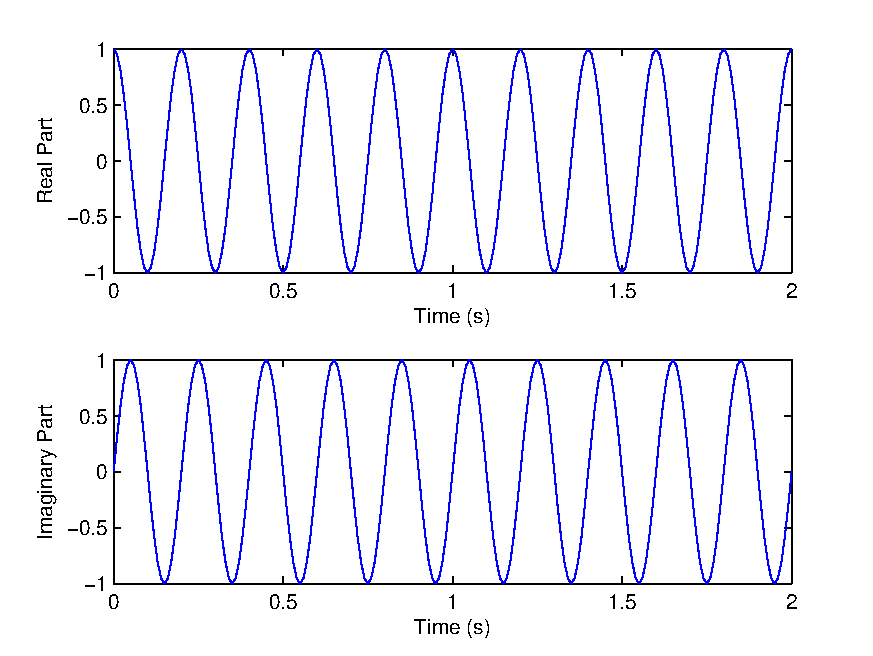
\includegraphics{hw1_1_2a-eps-converted-to.pdf}
        \end{center}
    Breaking \(h(t)\) into real and imaginary parts gives \(h(t) = \cos(10\pi t) + j\sin(10\pi t)\).
    \end{feedback}
\end{problem}

\begin{problem}
    Use \texttt{subplot} to plot the magnitude and phase of \(h(t)\).
    Use the command \texttt{angle()} or \texttt{unwrap(angle())} to plot the phase.
    \begin{multipleChoice}
        \choice[correct]{I've done this.}
        \choice{I have not done this.}
    \end{multipleChoice}
    \begin{feedback}[correct]
        \begin{center}
            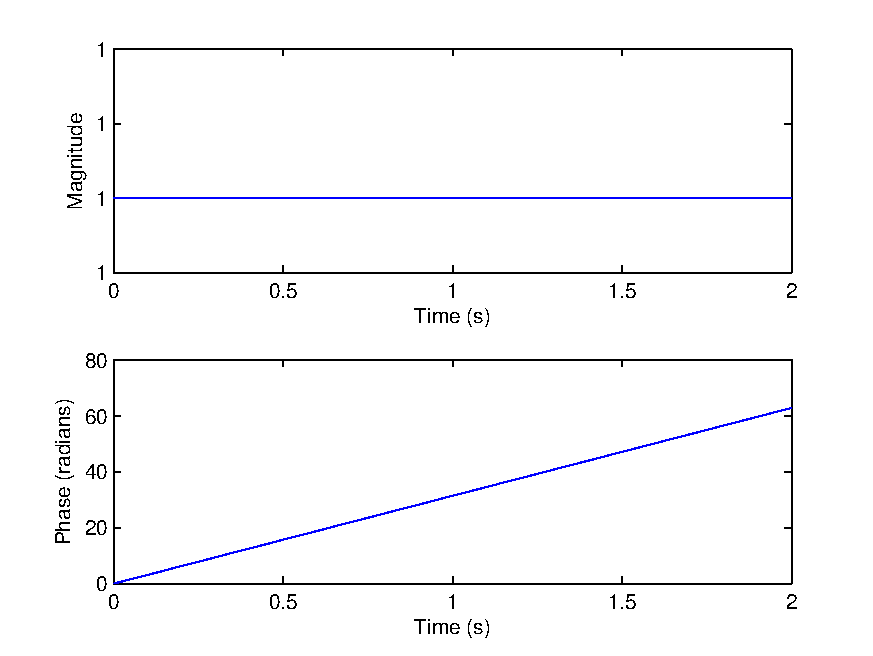
\includegraphics{hw1_1_2b-eps-converted-to.pdf}
            \end{center}
    The magnitude is constant, while the phase varies periodically as computed using \texttt{angle()}.
    \end{feedback}
\end{problem}
\end{document}